\chapter{Complessità computazionale}\label{chap:CC}
L'obiettivo della complessità computazionale è quello di catalogare i vari problemi in base alla loro complessità intrinseca e di quantificare le risorse computazionali richieste per la loro risoluzione.
Per risorse computazionali si intendono il tempo necessario per terminare una computazione, la quantità di gate o di memoria richieste per eseguire un algoritmo o, meno frequentemente, l'energia necessaria per risolvere un problema.
Questa volontà è motivata dal desiderio degli uomini di individuare le classi dei problemi facilmente risolubili, ovvero per cui esiste un algoritmo efficiente, e dei problemi facilmente verificabili, ovvero per cui esiste una configurazione che certifica la risolubilità del problema.
Per analizzare le richieste è necessario fissare un sistema computazionale su cui eseguire gli algoritmi.
In base ad esse, poi, si definiscono le classi di complessità in cui sono divisi i problemi.
Lo scopo delle prossime sezioni sarà di introdurre i due principali modelli computazionali, ai fini della computazione quantistica: la macchina di Turing e i circuiti quantistici.
Su di essi si definiranno, poi, le più importanti classi di complessità, tra cui le celeberrime \textbf{P} -- classe dei problemi risolubili in modo efficiente -- ed \textbf{NP} -- classe dei problemi facilmente verificabili -- e le controparti quantistiche \textbf{BQP} e \textbf{QMA}.

\section{Macchine di Turing}
Le macchine di Turing sono un modello computazionale classico di enorme rilevanza storica e teorica.
Esse sono strumenti semplici, ma estremamente potenti e versatili.
Per giustificarne l'inclusione in questa trattazione si è scelto di anteporre alla loro definizione una famosa tesi che vuole rendere più chiara la potenza computazionale di tale modello:

\begin{description}[align=left]
  \item [Tesi di Church-Turing:] La classe di funzioni computabili da una macchina di Turing corrisponde alla classe di funzioni che possono essere calcolate seguendo un algoritmo.
\end{description}
\noindent
Questa tesi non è un teorema e non può essere dimostrata, in quanto sarebbe necessario definire in modo preciso la classe di funzioni calcolabili tramite un algoritmo.
Quello che, invece, vuole affermare è l'uguaglianza tra la precisa nozione della classe di funzioni calcolabili da una macchina di Turing e l'insieme delle funzioni che, intuitivamente, si considerano computabili seguendo un algoritmo.
Giustifica, quindi, la scelta della macchina di Turing come modello computazionale di riferimento, capace di computare tutto ciò che può essere calcolato.
\subsubsection{Macchina di Turing}
Una \textit{macchina di Turing a $k$ nastri} è una macchina astratta dotata delle seguenti caratteristiche:
\begin{enumerate}[align=left]
 \item[\textbf{Spazio di lavoro:}] i $k$ nastri formano lo spazio di lavoro. Un nastro è una sequenza monodimensionale, infinita a destra, di celle. 
 Ogni cella può contenere un elemento di un alfabeto $\Gamma$.
 Su ogni nastro è presente una testina che può leggere o scrivere sulla cella su cui è posizionata. 
 La computazione avviene in intervalli temporali discreti in cui, in ciascun intervallo, le testine possono muoversi al più di una posizione, a destra o sinistra, sul proprio nastro.
 
 In particolare il primo nastro è il nastro di \textit{input}, contenente i dati del problema. 
 È un nastro di sola lettura e la testina non può scrivere su esso.
 Gli altri, invece, sono i nastri di lavoro, sui quali le testine possono anche scrivere.
 Uno di questi viene dedicato all'\textit{output}, ed è il nastro da cui si legge il risultato della computazione quando la macchina di Turing si arresta.
 
 \item[\textbf{Insieme di regole operative:}] una macchina di Turing può trovarsi in un qualunque stato di un fissato insieme, detto $Q$. 
 Tra questi saranno presenti $q_{\mathsf{start}}$, assunto dalla macchina a inizio computazione, e $q_{\mathsf{halt}}$, che segnala il termine delle operazioni.
 Lo stato in cui si trova determina il comportamento della macchina di Turing.
 Infatti, essa opera nel seguente modo: 
 (1) le $k$ testine leggono il contenuto della cella su cui si trovano, 
 (2) in base allo stato della macchina le $k-1$ testine scrivono sulla cella un nuovo simbolo dell'alfabeto,
 (3) sempre in base allo stato, le varie testine si muovono a destra o sinistra, al più di una posizione,
 (4) la macchina di Turing cambia stato, scegliendo dall'insieme $Q$.
\end{enumerate}
Formalmente una macchina di Turing è definita da
\begin{defn}[Macchina di Turing]\label{defn:TM}
 Una {\upshape macchina di Turing} $M$ a $k$ nastri è una tripletta ordinata $\left(\Gamma, Q, \delta \right)$, dove:
 \begin{itemize}
  \item $\Gamma$ è l'insieme, detto {\upshape alfabeto} di $M$, con i simboli che possono essere salvati nelle celle dei nastri.
  Contiene i simboli $\square$, che indica la cella vuota, e $\rhd$, che indica l'inzio del nastro.
  \item $Q$ è l'insieme degli {\upshape stati} in cui può trovarsi $M$.
  Vi appartengono gli stati $q_{\mathsf{start}}$ e $q_{\mathsf{halt}}$, che rappresentano l'inizio e la fine della computazione.
  \item $\delta: Q \cross \Gamma^k \to Q \cross \Gamma^{k-1} \cross \left\{\mathsf{L}, \mathsf{S}, \mathsf{R}\right\}^k$ è detta {\upshape funzione di transizione} e regola il comportamento della macchina di Turing.
 \end{itemize}
\end{defn}
Il comportamento della macchina di Turing $M$ è determinato da $\delta$ nel seguente modo:
siano $q \in Q$ lo stato di $M$ e $\left(\sigma_1, \sigma_2, \dots, \sigma_k \right)$ i simboli letti sui $k$ nastri.
Sia $\left(q', (\sigma'_2, \dots, \sigma'_k), z\right) := \delta\left(q, (\sigma_1, \sigma_2, \dots, \sigma_k) \right)$, dove $z \in \left\{\mathsf{L}, \mathsf{S}, \mathsf{R}\right\}^k$ l'immagine di $\delta$.
Al prossimo passo della computazione $M$ passerà allo stato $q'$, le $k-1$ testine sui nastri di lavoro scriveranno $(\sigma'_2, \dots, \sigma'_k)$ sulla propria cella e, infine, le $k$ testine si muoveranno in base al corrispondente valore di $z$: se è $\mathsf{L}$ a sinistra, $\mathsf{R}$ a destra mentre con $\mathsf{S}$ non si muovono.
Si assume che una testina, se è sulla prima cella e la mappa $\delta$ le impone di muoversi a sinistra, non si muoverà.

La computazione di $M$, fissata una stringa di input $x$, avviene secondo il seguente schema.
Tutti i nastri, a meno di quello di input, sono inizializzati con il simbolo $\rhd$ sulla prima cella e ogni altra cella vuota, ovvero con il simbolo $\square$.
Il nastro di input è inizializzato con la prima cella a $\rhd$, seguita da una sequenza finita di celle non vuote, che rappresentano l'input $x$, e il resto con il simbolo $\square$.
A inizio computazione tutte le testine sono sulla cella più a sinistra -- con il simbolo $\rhd$ -- e $M$ è nello stato $q_{\mathsf{start}}$. Questa è chiamata configurazione iniziale di $M$ sull'input $x$.

Da questa configurazione iniziale la computazione segue il procedimento codificato da $\delta$, come descritto in precedenza, fino a che non raggiunge lo stato $q_{\mathsf{halt}}$.
In questo stato la funzione di transizione è definita per non modificare ulteriormente la configurazione della macchina $M$.
Si è, quindi, fermata la computazione e si può leggere l'output nel nastro designato.

Non è necessario che la macchina di Turing arrivi mai allo stato $q_{\mathsf{halt}}$. Potrebbe, infatti, non terminare mai la computazione e non restituire mai un output completo.

Si introduce, quindi, la seguente notazione: Fissata una macchina di Turing $M$ e un input $x$, si definisce:
\begin{align}
 M(x) := 
 \begin{cases}
  y & \text{se } M \text{ raggiunge lo stato } q_{\mathsf{halt}}\\
  \nearrow & \text{altrimenti}
 \end{cases},
\end{align}
dove, nel primo caso, $y$ è la stringa letta sul nastro di output quando la macchina di Turing raggiunge lo stato $q_{\mathsf{halt}}$.

\subsection{Codifica}
\begin{defn}[stringa binaria]
 Si definisce stringa binaria di lunghezza $n$ un elemento di $\left\{0,1\right\}^n$.\\
 L'insieme di tutte le stringhe binarie è $\left\{0,1\right\}^* := \cup_{n\geq0}\left\{0,1\right\}^n$.
\end{defn}
In genere, nello studio della complessità computazionale, si considerano solamente funzioni il cui dominio e codominio sono stringhe binarie.
Si possono rappresentare funzioni su oggetti arbitrari tramite questo tipo di mappe.
Per raggiungere questo scopo bisogna definire una \textit{codifica}, ovvero una mappa iniettiva dall'insieme contenente tutti gli oggetti su cui si vuole operare, a valori nell'insieme delle stringhe binarie $\left\{0,1\right\}^*$.
L'unica richiesta che si pone è che a oggetti distinti corrispondano stringhe distinte.

Vista questa consuetudine si tendono a considerare macchine di Turing il cui alfabeto è $\Gamma := \left\{\square, \rhd, 0, 1\right\}$.
Fissato un problema, poi, si specifica una codifica in cui rappresentare la classe di oggetti su cui si opera. Nel prosieguo della trattazione, infatti, si assumerà sempre l'utilizzo di tale alfabeto e, se necessario, sarà anche introdotta la codifica usata.

\section{Problemi decisionali}
Una particolare classe di problemi studiati nella teoria della complessità computazionale sono i cosiddetti \textit{problemi decisionali}, associati ai \textit{linguaggi}.
Essi permettono di costruire un'elegante famiglia di classi di complessità e, per questo motivo, sono spesso usati in letteratura.
Per arrivare alla definzione di linguaggio è necessario introdurre il concetto di stringa su alfabeti arbitrari, non solo binaria:
\begin{defn}[Insieme delle stringhe]
 Dato un insieme finito $\Sigma$, detto alfabeto, si dice stringa di lunghezza $n$, sull'alfabeto $\Sigma$, un elemento di $\Sigma^n$.\\
 L'insieme di tutte le stringhe sull'alfabeto $\Sigma$ è $\Sigma^* := \cup_{n\geq0}\Sigma^n$.
\end{defn}
Con questa nozione si introduce il concetto di linguaggio:
\begin{defn}[Linguaggio]
 Dato un'alfabeto $\Sigma$ si definisce {\upshape linguaggio} un sottoinsieme $L \subset \Sigma^*$ delle stringhe sull'alfabeto $\Sigma$.
\end{defn}
Il problema decisionale associato chiede di decidere se, dato un arbitrario $x \in \Sigma^*$, si ha $x \in L$ oppure no.
Si dice che $x$ è una soluzione al problema decisionale, o verifica il problema, sse $x \in L$.

È importante notare che ogni linguaggio può essere associato a una funzione Booleana -- ovvero il cui codominio è $\{0,1\}$ -- e viceversa.
La prima associazione si ottiene definendo $f: X \to \{0,1\}$ in modo che $f(x) = 1 \iff x \in L$, ovvero $L = \left\{x \in X : f(x) = 1\right\}$.
Data una funzione Booleana sull'insieme $X$, analogamente, si definisce il linguaggio associato $L_f := \left\{x \in X : f(x) = 1\right\}$.

Si possono utilizzare le macchine di Turing per \textit{decidere} i linguaggi, ovvero per verificare se, dato un linguaggio $L$, un determinato elemento $x$ appartiene a $L$.
Per far ciò si introduce un'opportuna codifica $c$, che mappi $L$ in $\left\{0,1\right\}^*$, in modo da ottenere un analogo linguaggio $c(L) \subseteq \left\{0,1\right\}^*$.
Si dice, ora, che una macchina di Turing $M$ \textit{decide} o \textit{risolve} il linguaggio $L$ sse
\begin{equation}
 M(x) = 
 \begin{cases}
  1     & \text{se } x \in c(L)\\
  0     & \text{se } x \notin c(L)
 \end{cases},
\end{equation}
ovvero se, per ogni stringa $x$ in input, $M$ arriva allo stato $q_{\mathsf{halt}}$ in un tempo finito.
In particolare la macchina $M$, in un tempo finito, afferma che il valore in input è, o non è, una soluzione al probelma decisionale $L$.

Una condizione più debole, ma comunque utile, chiede che
\begin{equation}
 M(x) = 1 \quad \forall \, x \in c(L).
\end{equation}
In tal caso si dice che la macchina $M$ \textit{accetta} $L$.
La condizione è più debole in quanto, se $x \notin c(L)$, non si richiede nemmeno che $M$ termini la computazione, potrebbe essere $M(x) = \nearrow$.
Questa condizione è più naturale per codifiche di linguaggi, in quanto, dato un linguaggio $L \subseteq X$, in genere esistono stringhe $x \notin c(X)$.

\section{Richieste computazionali}
Per analizzare la complessità di un problema è necessario, innanzitutto, definire una grandezza che rappresenti la richiesta di risorse computazionali di un dato algoritmo o di una data macchina di Turing.

La prima risorsa considerata è il tempo.
Nel caso di macchine di Turing può essere facilmente definito il \textit{tempo di computazione} contando le operazioni elementari necessarie a giungere allo stato $q_{\mathsf{halt}}$.

È chiaro che questa quantità varia con l'input considerato.
Si può, infatti, ottenere una funzione che associ ad ogni diversa stringa di input il tempo necessario per il completamento della computazione.
Risulta più interessante, però, studiare il tempo richiesto in funzione della lunghezza della stringa in input.
Fissata una lunghezza, però, non è più univocamente determinato il tempo di computazione di una macchina di Turing. 
Bisogna, quindi, operare una scelta su che tempo considerare.
In genere si tende a scegliere il tempo massimo, che porta a formulare le seguenti definizioni:
\begin{defn}[Tempo di calcolo e computazione]\label{defn:running_time}
 Siano $f: \left\{0,1\right\}^* \to \left\{0,1\right\}^*$ e $T: \N \to \N$ due funzioni.
 Sia $M$ una macchina di Turing.
 Si dice che $M$ {\upshape computa} $f$ in tempo $T(n)$ o $T$ sse per ogni $x \in \left\{0,1\right\}^*$ la macchina $M$, con input $x$, dopo al più $T(|x|)$ passi, arriva allo stato $q_{\mathsf{halt}}$ con $f(x)$ stampato sul nastro di output.
 
 Si dice che $M$ {\upshape computa} $f$ sse esiste una tale funzione $T$ per cui $M$ computa $f$ in tempo $T$.
\end{defn}
Nella definizione precedente si è usata la notazione $|x|$ per indicare la lunghezza della stringa $x$.

In maniera analoga si può definire il tempo di calcolo per le macchine di Turing o persino per i linguaggi.
Si dice, infatti, che una macchina $M$ opera in tempo $T: \N \to \N$ sse, per ogni input $x \in \left\{0,1\right\}^*$, $M$ raggiunge lo stato $q_{\mathsf{halt}}$ in al più $T(|x|)$ passi.
Analogamente un linguaggio $L$ è deciso in tempo $T(n)$ sse esiste una macchina di Turing $M$ che decide $L$ e opera in tempo $T$.

L'esatto comportamento di $T$, però, risulta spesso superfluo, soprattutto per dati in input di grandi dimensioni.
È, infatti, sufficiente conoscerne il termine che cresce più velocemente per poter confrontare algoritmi e problemi distinti.

Inoltre, cambiando leggermente il modello su cui eseguire la computazione, per esempio aggiungendo lettere all'alfabeto di una macchina di Turing, il singolo algoritmo viene eseguito in tempi diversi. Spesso questa differenza è la sola moltiplicazione per una costante, che non influisce sulla scala degli infiniti.

Per tenere conto di queste richieste si introduce la seguente notazione.

\begin{defn}[notazione asintotica]\label{defn:Oh_notation}
 Siano $f,g : \N \to \R$, si introducono le seguenti notazioni:
 \begin{description}[align=left]
  \item [$O$ grande:] Si dice che $f$ è $O$ grande di $g$, notazione $f = O(g)$, sse 
  \begin{equation}
   \exists\, n_0 \in \N \text{, } c \in \R \text{ t.c. } f(n) \leq cg(n)\quad \forall \, n \geq n_0.
  \end{equation}
  \item [$\mathbf{\Omega}$ grande:] Si dice che $f$ è $\Omega$ grande di $g$, notazione $f = \Omega(g)$, sse 
  \begin{equation}
   \exists\, n_0 \in \N \text{, } c \in \R \text{ t.c. }  cg(n) \leq f(n) \quad \forall \, n \geq n_0.
  \end{equation}
  \item [$\mathbf{\Theta}$ grande:] Si dice che $f$ è $\Theta$ grande di $g$, notazione $f = \Theta(g)$, sse
  \begin{equation}
   f = O(g) \text{ e } f = \Omega(g)
  \end{equation}
 \end{description}
\end{defn}
Le tre notazioni hanno finalità distinte, ma tutte legate al confronto delle richieste computazionali di algoritmi e problemi distinti.

$O$ grande è usato per confrontare algoritmi differenti.
Permette di trovare una semplice, ma sufficientemente accurata, maggiorazione delle richieste computazionali di un dato algoritmo. 
Essendo una maggiorazione consente di confrontare le richieste massime degli algoritmi, permettendo un'ordinamento semplice di essi.

$\Omega$ grande, invece, è utilizzato per studiare interi problemi, indipendentemente dall'algoritmo usato per risolverli, oppure classi di algoritmi.
In queste analisi, infatti, è utile individuare minorazioni alle richieste computazionali, per avere una stima della difficoltà del problema, oppure dell'efficienza della classe scelta di algoritmi.

$\Theta$ grande, invece, permette di individuare algoritmi che hanno lo stesso comportamento asintotico.
Un semplice esempio consiste di implementazioni dello stesso algoritmo in differenti modelli computazionali.

\section{Classi di complessità}
Una classe di complessità è un insieme di problemi decisionali che possono essere decisi, in un dato modello computazionale, entro un fissato limite di risorse.
Le prime che saranno definite useranno il modello della macchina di Turing e considereranno limiti sul tempo di computazione.

Si costruisce, innanzitutto, l'importante classe \textbf{P} la quale, intuitivamente, rappresenta i problemi che ammettono una soluzione efficiente.
\subsection{Tempo deterministico e P}
Sfruttando la definizione \ref{defn:running_time} per il tempo di calcolo, si introducono le classi di tempo deterministico:
\begin{defn}[classe \textbf{DTIME}]\label{defn:DTIME}
 Sia $T: \N \to \N$ una funzione.
 Si definisce \textbf{DTIME}$(T)$ la classe di ogni problema decisionale $L$ per il quale esiste una costante $c > 0$ t.c. $L$ è deciso in tempo $c \cdot T$.
\end{defn}
La classe \textbf{DTIME}$(T)$, quindi, rappresenta tutti i linguaggi $L$ per cui esiste una macchina di Turing $M$ che decide $L$ in tempo $t = O(T)$. Si può, quindi, dire che la richiesta di tempo del problema $L$ è $O(T)$.

In base alla precedente definizione si può costruire la classe dei problemi decidibili in modo efficiente, ovvero con richiesta di tempo polinomiale:
\begin{defn}[classe \textbf{P}]\label{defn:P}
 Si definisce \textbf{P}$:= \cup_{c\geq 1}$\textbf{DTIME}$(n^c)$.
\end{defn}
Questa classe gioca un ruolo importantissimo nella teoria della complessità computazionale, quindi merita alcune osservazioni.
Tramite questa classe si definiscono, infatti, i problemi che ammettono risoluzione efficiente e, a priori, non è ovvio il motivo.
Pare strano che un problema la cui richiesta di tempo sia di $O(n^{1000})$ possa essere considerato efficiente.
Inoltre le costanti non esplicitate potrebbero rendere un problema in \textbf{DTIME}$(e^n)$ sostanzialmente più veloce da risolvere, per piccoli input, di un problema in \textbf{DTIME}$(n^2)$.
Nonostante questi criticismi, risulta effettivamente una buona scelta definire la classe dei problemi risolubili in modo efficiente tramite \textbf{P}.

Da un punto di vista più pratico si potrebbe, infatti, decidere, di chiamare efficiente un dato algoritmo che sia computabile in tempo, per esempio, $n^2$.
Sarebbe naturale definire efficienti anche algoritmi che eseguono solamente operazioni efficienti con al più chiamate ad altri algoritmi efficienti.
Permettendo questo innestamento si individua esattamente \textbf{P} come classe dei problemi che ammettono risoluzioni efficienti.

Si potrebbe anche criticare, a questa definizione di problema efficientemente risolubile, la dipendenza da uno specifico modello computazionale.
Nulla garantisce che i problemi in \textbf{P} siano efficientemente risolubili in modelli computazionali come i circuiti classici o quantistici, per non citare modelli più esotici.
Tuttavia esiste una forma forte della tesi di Church-Turing, che vuole risolvere proprio questo problema.
\begin{description}[align=left]
  \item [Tesi forte di Church-Turing:] Ogni modello computazionale fisicamente realizzabile può essere simulato da una macchina di Turing con al più un incremento polinomiale nelle richieste computazionali.
\end{description}
La veridicità di questa tesi, infatti, garantirebbe la buona definizione classe \textbf{P} come classe dei problemi efficientemente risolubili.
Essa risulterebbe, infatti, indipendente dal modello computazionale.

\subsection{Classe NP e tempo non deterministico}
La seguente classe svolge un ruolo strettamente legato ai problemi che ammettono soluzione efficiente.
Si tratta, infatti, dei problemi per i quali si può verificare in modo efficiente la veridicità di una soluzione.
In termini più precisi: sono i problemi decisionali per i quali, dato un $x$ che verifica il problema -- ovvero che è nel linguaggio -- si ha una stringa di dimensioni non troppo grandi che certifica in modo efficiente l'appartenenza di $x$ in $L$.
La definizione formale è la seguente:
\begin{defn}[classe NP]\label{defn:NP_det}
 Si definisce \textbf{NP} la classe contenente tutti i linguaggi $L \subseteq \left\{0,1\right\}^*$ tali per cui esistono un polinomio $p: \N \to \N$ e una macchina di Turing $M$, di tempo polinomiale, tali che, per ogni $x \in \left\{0,1\right\}^*$:
 \begin{equation}
  x \in L \iff \exists u \in \left\{0,1\right\}^{p(|x|)} \text{ t.c. } M(x,u) = 1
 \end{equation}
\end{defn}
Se $x \in L$, ogni $u \in \left\{0,1\right\}^{p(|x|)}$ che soddisfa $M(x,u)=1$ viene detto certificato per $x$ (rispetto al linguaggio $L$ e alla macchina di Turing $M$).

Questa è la prima definizione che sarà data di \textbf{NP} e risulta più intuitiva più intuitiva della successiva.
L'importanza di questa definizione, ai fini pratici, può essere spiegata con l'esempio della crittografia.
Si vuole, infatti, che il problema di decifrare un messaggio crittato sia in \textbf{NP}.
Fissati un messaggio cifrato e in chiaro, la situazione migliore sarebbe che, senza ulteriori informazioni, il problema di decidere se il primo viene decodificato nel secondo sia difficile.
Si vuole, però, che il possessore della chiave di cifratura possa verificare l'affermazione precedente in modo efficiente.
La chiave di cifratura, dunque, opererebbe da certificato, rendendo facile il controllo.

Il fatto che esistano dei tali problemi, che siano effettivamente difficili da risolvere in mancanza del certificato, ma facili in sua presenza, è ancora un problema irrisolto.
Per risolverlo è necessario studiare la relazione insiemistica che lega \textbf{P} ed \textbf{NP}, argomento approfondito nella prossima sezione.

Si presentano degli ulteriori esempi, basati sulla precedente definizione, per chiarificare il concetto di problema in \textbf{NP}:
\begin{enumerate}[align=left]
 \item[\textbf{Somma parziale:}] data una sequenza di $n$ numeri $a_1, \dots, a_n$ e un valore $S$, decidere se esiste una sottosequenza di $a_1, \dots, a_n$ la cui somma è $S$. Il certificato è la sequenza di numeri.
 \item[\textbf{Commesso viaggiatore:}] i dati sono un insieme di $n$ nodi, $\binom{n}{2}$ numeri $d_{i,j}$, i quali indicano la distanza tra i nodi $i$ e $j$, e un numero $k$.
 Il problema chiede di decidere se esiste un circuito chiuso che visita ogni nodo e che sia lungo al più $k$.
 Il certificato è il circuito.
 \item[\textbf{Numero composito:}] dato un numero $N$ decidere se è un numero composito o primo.
 Il certificato è la fattorizzazione di $N$.
 \item[\textbf{Fattorizzazione:}] dati tre numeri $N, L, U$ decidere se $N$ ammette un fattore $M$ nell'intervallo $\left[L,U\right]$.
 Il certificato è il fattore $M$ di $N$.
\end{enumerate}

Prima di analizzare le relazioni tra le classi di complessità appena definite è utile introdurre un nuovo modello computazionale e una definizione equivalente di \textbf{NP}:

\subsubsection{Macchina di Turing non deterministica}
Riprendendo la definizione \ref{defn:TM} di macchina di Turing si introduce la seguente:
\begin{defn}[Macchina di Turing non deterministica]\label{defn:NDTM}
 Una macchina di Turing non deterministica $N$ a $k$ nastri è una tripletta ordinata $\left(\Gamma, Q, \delta \right)$, dove:
 \begin{itemize}
  \item $\Gamma$ è l'insieme, detto {\upshape alfabeto} di $N$, con i simboli che possono essere salvati nelle celle dei nastri.
  Contiene i simboli $\square$, che indica la cella vuota, e $\rhd$, che indica l'inzio del nastro.
  \item $Q$ è l'insieme degli {\upshape stati} in cui può trovarsi $N$.
  Vi appartengono gli stati $q_{\mathsf{start}}$ e $q_{\mathsf{halt}}$, che rappresentano l'inizio e la fine della computazione.
  \item $\delta \subseteq \left[Q \cross \Gamma^k\right] \cross \left[Q \cross \Gamma^{k-1} \cross \left\{\mathsf{L}, \mathsf{S}, \mathsf{R}\right\}^k \right]$ è detta {\upshape relazione di transizione} e regola il comportamento della macchina di Turing.
 \end{itemize}
\end{defn}
Come nel caso deterministico si usa il primo nastro come solo input, l'ultimo come nastro di output e gli altri come nastri di lavoro.
L'unica differenza dalla definizione \ref{defn:TM} consiste nel fatto che $\delta$ non è più una funzione, ma una relazione.
In questo dettaglio risiede il non determinismo del nuovo modello computazionale. Infatti, a partire da una data configurazione di $N$ -- stato della macchina, posizione delle testine e contenuti dei nastri -- non è determinato in modo univoco la configurazione seguente.
Fissata una prima configurazione, infatti, si apre un albero, che rappresenta le possibili evoluzioni della computazione, come rappresentato nella figura \ref{fig:Conf_tree}.
Tale differenza dal modello deterministico comporta una nozione completamente differente di risoluzione di un problema decisionale.
Infatti si dice che la macchina di Turing non deterministica $N$ decide il problema decisionale $L$ sse: (1) per ogni $x \in L$ esiste una successione di scelte non deterministiche che risulta in una computazione in cui $N$ raggiunge lo stato $q_{\mathsf{halt}}$ e riporta sul nastro di output $1$, (2) per ogni $x \notin L$ non esiste alcuna sequenza di scelte come descritte nel caso (1).

Si ha un comportamento asimmetrico tra (1) e (2), simile alla definizione di accettazione di un linguaggio da parte di una macchina di Turing deterministica $M$.

\begin{figure}[h]
\begin{center}
 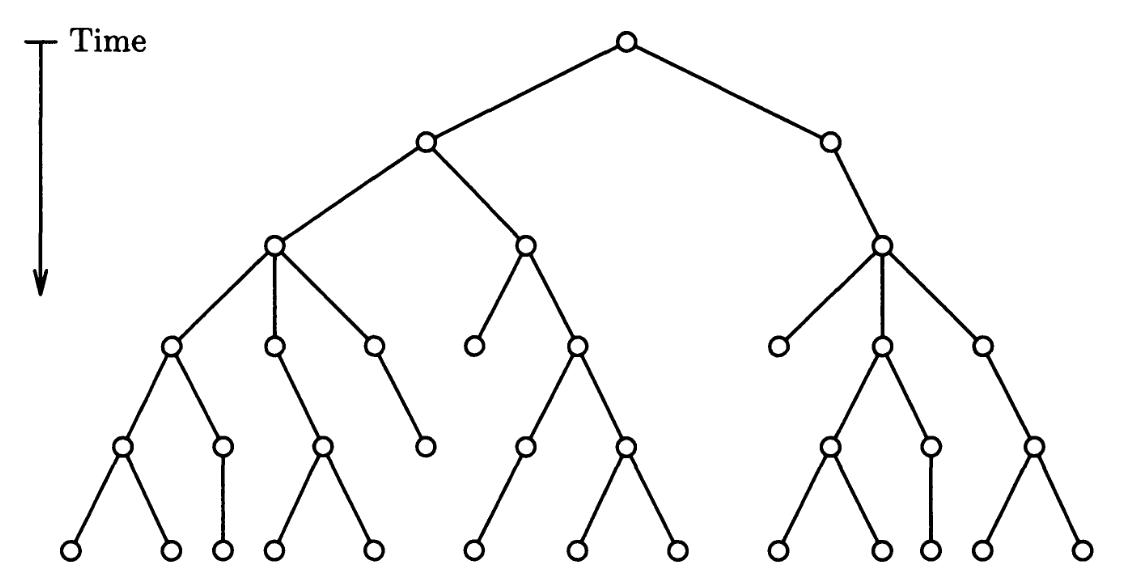
\includegraphics[width=\textwidth]{Images/Albero_configurazioni}
\end{center}
\caption{Computazione non deterministica.}\label{fig:Conf_tree}
\end{figure}

Si dice, inoltre, che una macchina di Turing non deterministica $N$ decide il linguaggio $L$ in tempo $T: \N \to \N$ sse $N$ decide $L$ e, per ogni stringa $x$ in input, ogni possibile scelta non deterministica porta a computazioni che raggiungono lo stato $q_{\mathsf{halt}}$ in un numero di passi $k \leq T(|x|)$.
Nella rappresentazione grafica $T(|x|)$ è una maggiorazione della profondità dell'albero delle possibili computazioni non deterministiche.
È interessante notare che, ad un fissato livello di profondità, il modello di macchina di Turing non deterministica esplora un insieme di possibili configurazioni esponenzialmente più grande rispetto alla macchina di Turing deterministica.

Si possono, ora, introdurre le classi di tempo non deterministico:
\begin{defn}[classe \textbf{NTIME}]\label{defn:NTIME}
 Sia $T: \N \to \N$ una funzione.
 Si definisce \textbf{NTIME}$(T)$ la classe di ogni problema decisionale $L$ per il quale esistono una costante $c > 0$ e una macchina di Turing non deterministica $N$ t.c. $N$ decide $L$ in tempo $c \cdot T$.
\end{defn}
Ovvero la trasposizione non deterministica della definizione \ref{defn:DTIME}.
In queste due definizioni, infatti, \textbf{D} indica il determinismo e \textbf{N} il non determinismo del modello computazionale utilizzato.

Si può dare, analogamente al caso di \textbf{P}, la definizione di problema risolubile in tempo polinomiale da una macchina non deterministica.
In questo caso -- come storicamente -- \textbf{NP} indica Non deterministic \textbf{P}.
\begin{defn}[classe \textbf{NP$_\mathbf{s}$}]\label{defn:NP_Ndet}
 Si definisce \textbf{NP$_\mathbf{s}$}$:= \cup_{c\geq 1}$\textbf{NTIME}$(n^c)$.
\end{defn}
Si è scelto il pedice \textbf{s} per indicare che questa è la definizione storica della classe \textbf{NP}.
Si hanno, ora, due definizioni indipendenti di \textbf{NP}, le quali risultano equivalenti:
\begin{thm}[equivalenza delle definizioni di \textbf{NP}]
 \textbf{NP$_\mathbf{s}$ = NP}
\end{thm}
\begin{proof}
 La dimostrazione si basa sul fatto che la successione di scelte che porta la macchina di Turing non deterministica a verificare l'input $x$ può essere usata come un certificato.
 \begin{enumerate}[align=left]
  \item[\textbf{NP$_\mathbf{s}$ $\subseteq$ NP:}] Sia $L \in$ \textbf{NP$_\mathbf{s}$}, allora esistono un polinomio $q: \N \to \N$ e una macchina di Turing non deterministica $N$ tali che per ogni input $x$, in un numero di passi inferiore a $q(|x|)$, $N$ giunge allo stato $q_{\mathsf{halt}}$.
  In particolare, se $x \in L$, per una particolare sequenza di scelte non deterministiche, $N$ stampa in output il valore $1$.
  Si consideri una codifica binaria della stringa che descrive le scelte.
  Se ne può individuare una tale che la lunghezza della codifica binaria sia al più $p(|x|) := c \cdot q(|x|)$ per ogni $x$, con $c \in \N$ una costante.
  
  Questa stringa opera come certificato per la definizione \ref{defn:NP_det}.
  Si può ora usare una macchina di Turing $M$ per simulare la macchina $N$, seguendo le scelte codificate dal certificato.
  Chiaramente questa simulazione può essere svolta con un solo incremento polinomiale nel tempo $q$ impiegato da $N$.
  $M$, in questo caso, verifica in tempo polinomiale che $x \in L$.
  Se, inoltre, $x \notin L$ si può prendere una qualsiasi sequenza di scelte non deterministiche e $M$ arriverà allo stato $q_{\mathsf{halt}}$, sempre in tempo polinomiale.
  La coppia $p$, $M$, dunque, soddisfa la definizione citata, per cui $L \in$ \textbf{NP}.
  
  \item[\textbf{NP$_\mathbf{s}$ $\supseteq$ NP:}] Sia $L \in$ \textbf{NP}, si considerino il polinomio $p: \N \to \N$ e la macchina di Turing $M$ come da definizione \ref{defn:NP_det}.
  Per ogni $x \in L$ esiste un certificato $u \in \left\{0,1\right\}^{p(|x|)}$ per cui $M(x,u)=1$.
  Si definisce la macchina di Turing non deterministica $N$ di $k+1$ nastri, dove $k$ è il numero di nastri di $M$, che opera nel seguente modo:
  Per le prime $p(|x|)$ operazioni scrive un carattere scelto casualmente tra $0$ e $1$ sul secondo nastro, poi opera deterministicamente.
  In particolare, nel secondo periodo, opera come la macchina di Turing $M$, considerando i primi due nastri come nastri di input (come se fossero concatenati).
  In quanto esiste un certificato $u$ di lunghezza $p(|x|)$ per cui $M(x,u)=1$, allora esiste una sequenza di scelte non deterministiche per cui $N$ stampa $u$ sul secondo nastro e arriva a stampare $1$.
  In quanto la macchina $M$ è polinomiale segue che anche $N$ lo sarà: esegue esattamente $p(|x|)$ operazioni più di quelle di $M$.
  Si è, quindi, verificato che $L \in$ \textbf{NP$_\mathbf{s}$}.\qedhere
 \end{enumerate}
\end{proof}

\subsection{Relazione tra P ed NP}
In quanto la definizione di macchina di Turing non deterministica è un'estensione di quella deterministica, risulta chiaro che ogni macchina di Turing $M$ è anche non deterministica (semplicemente non è molto interessante come tale).
È, quindi, chiaro che, per ogni funzione $T: \N \to \N$, si ha \textbf{DTIME}$(T) \subseteq$ \textbf{NTIME}$(T)$.
Da questo segue che \textbf{P} $\subseteq$ \textbf{NP}.

Purtroppo questo è il più raffinato risultato conosciuto per quanto riguarda la relazione tra \textbf{P} ed \textbf{NP}.
Uno dei $7$ problemi del millennio, infatti, chiede di stabilire se, effettivamente, \textbf{P} $\neq$ \textbf{NP}, ma rimane tutt'ora irrisolto.

Anche riprendendo i pochi esempi descritti nella sezione precedente si nota l'incompletezza delle informazioni a nostra disposizione:

\begin{enumerate}[align=left]
 \item[\textbf{Commesso viaggiatore:}] Si può dimostrare che è un problema di ``difficile'' soluzione.
 In particolare si dimostra che è in \textbf{P} sse \textbf{P} = \textbf{NP}.
 \item[\textbf{Numero composto:}] È stato recentemente mostrato, in \cite{Article:PRIMESinP}, che questo problema è in \textbf{P}.
 \item[\textbf{Fattorizzazione:}] Tutt'ora non si sa se sia, o meno, in \textbf{P} o se sia ``difficile'' quanto il problema del commmesso viaggiatore.
 Si suppone, assumendo \textbf{P} $\neq$ \textbf{NP}, che sia in \textbf{NP}$\setminus$\textbf{P}.
 È per questa ragione che esistono sistemi crittografici basati sul problema della fattorizzazione degli interi.
\end{enumerate}

\section{Classi di complessità quantistica}
Per ora è stata introdotta la sola teoria classica.
Per passare allo studio degli algoritmi che seguiranno è necessario formalizzare il modello dei circuiti, in particolare quantistici, e introdurre le definizioni, che riprendano quelle date nelle sezioni precedenti, per richieste computazionali e classi di complessità.

\subsection{Circuiti Booleani e complessità}
Nel primo capitolo si è data una nozione informale e operativa di circuito, per comprendere il funzionamento di un computer quantistico.
Segue una definizione più formale dei circuiti classici utilizzati per computare funzioni di Boole, associate ai problemi decisionali.
\begin{defn}[Circuito booleano]
 Si definisce {\upshape circuito booleano} con $n$ bit di input un grafo aciclico diretto nel quale i nodi possono essere:
 \begin{itemize}
  \item {\upshape nodi di input}, di grado entrante $0$, etichettati da uno degli $n$ bit dell'input,
  \item {\upshape porte logiche}, con grado entrante $1$ o $2$, scelte tra i gate \textsc{and}, \textsc{or} e \textsc{not}.
 \end{itemize}
 Tra questi nodi si sceglie un gate logico come porta di {\upshape output} del circuito.
\end{defn}
Ogni nodo con grado entrante maggiore di 1 è detto gate logico o porta logica.
Si indica con $C(x)$ l'output del circuito $C$ a partire dall'input $x$.
Si definiscono, inoltre, \textit{dimensione} del circuito il numero di porte logiche che possiede e \textit{profondità} del circuito la massima lunghezza di un cammino da una porta di input alla porta di output.

Risulta chiaro che, ogni circuito booleano con $n$ bit di input, computa una funzione booleana $f:\{0,1\}^n \to \{0,1\}$.
Si può, quindi, pensare di utilizzare dei circuiti per decidere linguaggi, o problemi decisionali.
In generale, però, un linguaggio -- o la sua codifica binaria -- contiene elementi di diversa lunghezza, per cui non basta un singolo circuito per decidere un intero linguaggio.
Si deve, infatti, introdurre la nozione di \textit{famiglia di circuiti}. 
Essa è una successione $\left\{ C_n \right\}_{n \in \N}$ di circuiti booleani, in cui il circuito $C_n$ opera su input di lunghezza binaria $n$.

Dato un linguaggio $L$, quindi, esiste sempre una famiglia di circuiti $\left\{ C_n \right\}_{n \in \N}$ che decide il linguaggio $L$, ovvero che ne computa la funzione booleana associata.
Si dice che questa famiglia è di \textit{dimensione minimale} (rispettivamente di \textit{profondità minimale}) se non esistono famiglie, che decidono lo stesso linguaggio, di dimensione (rispettivamente profondità) minore.

A partire da questi concetti, quindi, si dà la seguente definizione:
\begin{defn}[Complessità della dimensione dei circuiti]
 Dato un linguaggio formale $L$ si definisce {\upshape complessità della dimensione} dei circuiti la funzione $T: \N \to \N$, che associa ad ogni $n$ la dimensione di $C_n$, ovvero dell'$n$-esimo circuito della famiglia di dimensione minimale che decide $L$.
\end{defn}
Sostituendo profondità a dimensione si ottiene l'analoga definizione per la \textit{complessità di profondità} dei circuiti.

Il fatto che input di lunghezza diversa siano analizzati da circuiti distinti rende questo modello di computazione non uniforme.
A priori, infatti, in una famiglia di circuiti, non è richiesta alcuna relazione tra i vari elementi della famiglia.
Per studiare le classi di complessità originate da questo modello computazionale si introduce il concetto di uniformità.
Intuitivamente una famiglia è uniforme se esiste un algoritmo che descriva, in funzione della sola dimensione $n$ dell'input, come costruire il corrispondente circuito $C_n$.
Inoltre si distinguono vari tipi di uniformità in funzione delle risorse impiegate dall'algoritmo richiesto.

In particolare saranno utili le seguenti famiglie uniformi di circuiti (non solo booleani):
\begin{defn}[Famiglia uniforme in tempo polinomiale]\label{defn:Unif_family}
 Una famiglia di circuiti $\left\{ C_n \right\}_{n \in \N}$ si dice {\upshape uniforme in tempo polinomiale} sse esiste una macchina di Turing deterministica $M$ tale che:
 \begin{itemize}
  \item $M$ opera in tempo polinomiale,
  \item per ogni $n \in \N$ la macchina $M$ produce una descrizione del circuito $C_n$ sull'input della stringa contenente esattamente $n$ simboli $1$, denotata con $1^n$.
 \end{itemize}
\end{defn}

\subsection{Circuiti quantistici}\label{sec:QCircuits}
In analogia ai circuiti booleani si definiscono i circuiti quantistici:
\begin{defn}[Circuito quantistico]
 Si definisce {\upshape circuito quantistico} con $n$ qubit di input un grafo aciclico diretto nel quale i nodi possono essere:
 \begin{itemize}
  \item {\upshape nodi di input}, di grado entrante $0$, etichettati da uno degli $n$ qubit dell'input,
  \item {\upshape porte logiche}, con grado entrante uguale a quello uscente, scelte in una fissata famiglia di gate.
%  \item misure nella base computazionale, con grado uscente pari a quello entrante.
 \end{itemize}
 Di questi nodi si scelgono $m$ nodi con grado entrante maggiore di zero, ai quali si associa l'{\upshape output} del circuito.
\end{defn}
Dai nodi di output si vuole ottenere dell'informazione classica.
%Se il nodo scelto è una misura non si deve operare ulteriormente, altrimenti è necessario far seguire la porta logica da un'opportuna misura nella base computazionale.
È necessario, quindi, far seguire la porta logica di output da un'opportuna misura nella base computazionale, nell'implementazione del circuito.
Per un circuito $QC$ si indica l'output con $QC(x)$, dove $x$ è lo stato quantistico di input.
La famiglia di gate tra cui scegliere le porte logiche potrebbe essere finita o infinita.
Nella realizzazione fisica si è più portati a scegliere famiglie finite di porte logiche, per ovvie questioni pratiche.
A tal fine è importante lo studio di quelle che sono chiamate famiglie di gate universali, svolto in \cite{Book:QCQI}.
A differenza dei gate universali classici, che possono computare ogni funzione a valori in stringhe binarie, le famiglie universali quantistiche possono \textit{approssimare}, con arbitraria precisione, qualsiasi gate realizzabile.

Per scopi più teorici, invece, è utile considerare la famiglia infinita contenente tutti i gate su un singolo qubit e il gate \textsc{cnot}.
Essa, infatti, si dimostra essere sufficiente a simulare il comportamento di qualsiasi altro gate quantistico.
Per approfondire questo argomento si rimanda a \cite{Book:QCQI}.

\subsubsection{Classi di complessità}
Su questo modello computazionale si ripropongono, senza alterazioni, le nozioni di complessità della dimensione e della profondità dei circuiti.
Si riporta, per chiarezza, la prima:
\begin{defn}[Complessità della dimensione dei circuiti]
 Dato un linguaggio formale $L$ si definisce {\upshape complessità della dimensione} dei circuiti la funzione $T: \N \to \N$, che associa ad ogni $n$ la dimensione di $QC_n$, ovvero dell'$n$-esimo circuito della famiglia di dimensione minimale che decide $L$.
\end{defn}
Questa stima sarà spesso utilizzata nel capitolo seguente, per analizzare l'efficienza degli algoritmi sviluppati.
In particolare si userà la notazione asintotica descritta nella definizione \ref{defn:Oh_notation}.
Si dirà, dunque, che un algoritmo ha un costo computazionale di $O(T)$ gate per affermare che la corrispondente famiglia di circuiti ha complessità di dimensione $F = O(T)$.

Come per la complessità, anche i concetti di famiglia uniforme e, in particolare, di famiglia uniforme in tempo polinomiale, definizione \ref{defn:Unif_family}, si traspongono senza alterazione alcuna.

Si possono, ora, definire le classi di complessità quantistiche equivalenti a \textbf{P} ed \textbf{NP}.
La differenza principale con le precedenti, a meno del differente modello computazionale, risiede nella natura aleatoria della computazione quantistica. Si sarà, infatti, costretti a richiedere una minima probabilità di successo degli algoritmi.
\begin{defn}[classe BQP]\label{defn:BQP}
 La classe \textbf{BQP} contiene tutti i problemi decisionali $L$ che ammettono una famiglia uniforme in tempo polinomiale di circuiti quantistici $\left\{ QC_n \right\}_{n \in \N}$ tale che:
 \begin{itemize}
  \item Per ogni $n$ il circuito $QC_n$ prende in input $n$ qubit e restituisce in output un singolo bit,
  \item Per ogni $x \in L$ vale $\P\left(QC_{|x|}(x) = 1\right) \geq 2/3$
  \item Per ogni $x \notin L$ vale $\P\left(QC_{|x|}(x) = 0\right) \geq 2/3$
 \end{itemize}
\end{defn}
La sigla \textbf{BQP} rappresenta: ``Bounded-error Quantum Polynomial time''.
Si richiede, infatti, l'esistenza di una famiglia di circuiti, di cui si può ottenere una descrizione in tempo polinomiale tramite una macchina di Turing e che ha una probabilità di errore limitata.
Si noti che il valore $2/3$ è, fondamentalmente, simbolico.
La ripetizione, di un algoritmo che rispetti tale condizione, un numero costante di volte diminuisce esponenzialmente la probabilità di errore -- ogni ripetizione è indipendente -- rispettando comunque le condizioni della definizione.

Analogamente alla classe \textbf{P} si considerano i problemi in \textbf{BQP} come efficientemente risolubili da una computer quantistico.
Tutti gli algoritmi che verranno studiati nel prossimo capitolo soddisfano le condizioni appena esposte, ovvero risolvono problemi in questa classe di complessità.
Intuitivamente ciò è dovuto al fatto che si riesce a dare una descrizione esplicita dei circuiti che li implementano, indipendentemente dalla lunghezza degli input, in questa breve trattazione.

Mentre, come è reso evidente dai risultati trovati da Fredkin e Toffoli è noto che \textbf{P} $\subseteq$ \textbf{BQP}, attualmente non è conosciuta alcuna relazione tra le classi \textbf{NP} e \textbf{BQP}.
Ci sono, però, evidenze che \textbf{NP} $\nsubseteq$ \textbf{BQP}.
Inoltre, per quanto un computer quantistico possa essere fondamentalmente più veloce di un computer classico, è stato dimostrato che non sarà esponenzialmente più veloce di esso.

Si passa, ora, all'analogo quantistico di \textbf{NP}:
\begin{defn}[classe QMA]\label{defn:QMA}
 Si definisce \textbf{QMA} la classe contenente tutti i linguaggi $L \subseteq \left\{0,1\right\}^*$ tali per cui esistono un polinomio $p: \N \to \N$ e una famiglia uniforme in tempo polinomiale di circuiti quantistici $\left\{ QC_n \right\}_{n \in \N}$ tali che:
 \begin{align}
  \forall\, x \in L\ \exists \ket{\psi} \in \left(\C{2}\right)^{\otimes p(|x|)} \text{ t.c. }& \P\left( QC_{|x|}(\ket{x},\ket{u}) = 1 \right) \geq \frac{2}{3}\\
  \forall\, x \notin L\ , \forall\, \ket{\psi} \in \left(\C{2}\right)^{\otimes p(|x|)} \text{ si ha }& \P\left( QC_{|x|}(\ket{x},\ket{u}) = 1 \right) \leq \frac{1}{3}
 \end{align}
\end{defn}
Tale definizione riprende la definizione deterministica di problemi per i quali esiste un certificato efficientemente verificabile.
Come nel caso di \textbf{BQP} le differenze principali dalla definizione classica sono le seguenti.
Innanzitutto si ammette una probabilità di errore per la natura probabilistica della computazione quantistica.
Inoltre si richiede che il certificato sia di natura quantistica, ovvero un $p(|x|)$-qubit.
